% !TeX root = ../Thesis.tex

%************************************************
\chapter{Evaluation}\label{ch:evaluation}
%************************************************
\glsresetall % Resets all acronyms to not used

To answer the main question of this thesis, whether the integration of \glspl{NN} into \gls{VPR} can improve its performance, we optimize and thoroughly evaluate our system.

\section{Evaluation Scenario}

First describing our method of evaluation as well as the specific settings used, we then evaluate the various \gls{NN} candidates against each other to determine the best network structure. Following this, the original \gls{VPR} Placer is evaluated and compared with our versions integrating \glspl{NN}.

\subsection{Selected Benchmarks}\label{ch:benchmarks}

For the final evaluation we select three circuits from the \gls{VPR} benchmark suite that we did not use in any prior part of this project, namely \textit{mcml.blif}, \textit{or1200.blif}, and \textit{diffeq2.blif}. The circuits are selected quasi-randomly, but ensuring that at least each one \textit{big} and one \textit{small} circuit is chosen.

In the same manner we also select an \textit{evaluation} set of one circuit (\textit{raygentop.blif}), which we will need for our chosen method of model selection, detailed in \ref{ch:model-selection}. This set is intentionally small to keep the computational effort of model selection manageable.

As the \gls{VPR} Placement algorithm is a pseudo-randomized heuristic not guarantee to yield reproducible results (when starting from a different state), each evaluation on each of this circuits will be averaged over 3 redundant placing attempts with different random seeds to ensure robust results.

\subsection{Runtime/Quality Trade-off}

Our metric of choice is runtime/quality trade-off, specifically discretely sampled routing quality (minimum channel width and critical path length) for certain approximate absolute placement run-times. These run-times, or sampling points, are selected per benchmark circuit relative to the runtime of the unchanged \gls{VPR} Placer (t\textsubscript{p}) as:

\begin{itemize}
	\item 1   * t\textsubscript{p}, or \textit{normal-mode}
	\item 10  * t\textsubscript{p}, or \textit{slow-mode}
	\item 50  * t\textsubscript{p}, or \textit{very-slow-mode}
	\item \cite{TODO} values might change when eval. is performed
\end{itemize}

The actual run-time, while not A-Priori \textit{predictable} for a certain configuration of the modified \gls{VPR} Placer, can easily be \textit{controlled} with the \textit{inner\_num} setting of \gls{VPR}.\cite{vtr8} 

Based on observations we state without formal proof that most of the computations of the \gls{VPR} Placer are performed inside each of these steps. Furthermore, while steps perform random actions and can have vastly differing run-time, within a certain \textit{temperature level} steps with different run-times are distributed randomly, and the number of steps per temperature is generally high. Therefore, changing this number of steps will not change the distribution of step run-times within a certain temperature-level, which means their average run-time remains approximately the same. Therefore, changes to the \textit{inner\_num} parameter, which is a linear factor for the actual number of steps performed, affect the total runtime of the modified \gls{VPR} Placer approximately linearly.

By placing a benchmark circuit using a fixed setting for \textit{inner\_num}, we acquire the runtime at this setting. As early experiments showed that the runtime of the \gls{VPR} Placer using \glspl{NN} is one to two orders of magnitude slower than using \gls{HPWL}, this value is set to $0.01*num_blocks^(4/3)$, which equals one hundredth of the default value of the \gls{VPR} Placer. Therefore, this first check is estimated to take approximately as much time as the unchanged \gls{VPR} in \textit{normal-mode}.

Now, \textit{inner\_num} can be scaled appropriately to gain quality scores at each sampling point.

Evaluating the performance of a certain \gls{NN} during model selection consists of the following steps:

\begin{itemize}
	\item integration into \gls{VPR}
	\item determining the runtime over \textit{inner\_num}
	\item setting \textit{inner\_num} appropriately for \textit{slow-mode}
	\item placing the evaluation circuit three times
	\item routing each placement and logging average quality 
\end{itemize}

The final evaluation of the best \gls{CNN} and \gls{RNN} against unchanged \gls{VPR} is performed as follows:

\begin{itemize}
	\item integration into \gls{VPR}
	\item determining the runtime over \textit{inner\_num}
	\item setting \textit{inner\_num} appropriately for \textit{normal-mode}
	\item placing the test circuits three times
	\item routing each placement and logging average quality per circuit
	\item repeating for \textit{slow-mode} and \textit{very-slow-mode}
\end{itemize}

The thus computed quality/runtime trade-off is then compared with that of the unchanged \gls{VPR} Placer.

The \gls{VPR} Router primarily optimizes the \textit{channel width}, or maximum number of parallel routing channels used by the routing, by determining the minimum routable value via binary search. Therefore we select \textit{channel width} as the primary evaluation metric. In the final evaluation we will, however, also compare critical path lengths, as this, as \gls{VPR}'s secondary optimization target, defines the maximum operateable frequency of the circuit, directly influencing its computational capabilities.

\section{Model Selection}\label{ch:model-selection}

Although \glspl{NN} automatically tune their parameters to fit the target function, the structure and properties of the network itself has to be specified explicitly. While recent works try to automate even this, it is usually still necessary to manually design networks to achieve good results.

During model selection, \glspl{CNN} and \glspl{RNN} are evaluated independently from each other and using the same methodology. This yields a best \gls{CNN} and a best \gls{RNN}, which will both again be integrated into \gls{VPR} and evaluated against the unchanged Placer.  

\subsection{Empirical Model Search}

Typically, a first working design is found empirically through experimentation, based largely on best practices, related works, and intuition.\cite{TODO} In our case, the strict requirements on the runtime of the networks restricted the search space considerably, and the model candidates described in \ref{ch:cnn-design} and \ref{ch:rnn-design} represent the obvious choices for small and simple networks.

From these candidates, the best one is selected by evaluating each independently on evaluation data different from the training and the final test data, and comparing the results.

\subsection{\gls{HPO}}

\begin{figure}
	\begin{subfigure}[b]{0.45\linewidth}
		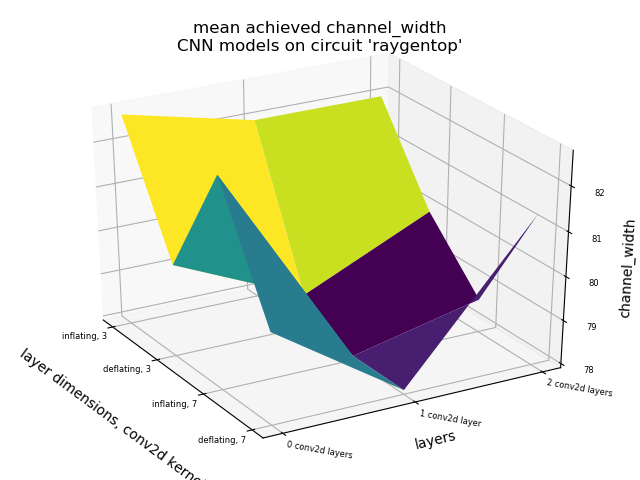
\includegraphics[width=\linewidth]{plots/cnn-hyperopt-chan-width.png}
		\caption{\glspl{CNN} - channel width}
	\end{subfigure}
	\begin{subfigure}[b]{0.45\linewidth}
		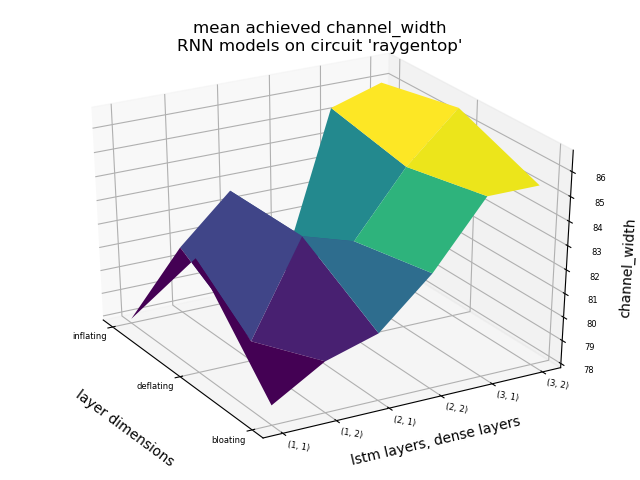
\includegraphics[width=\linewidth]{plots/rnn-hyperopt-chan-width.png}
		\caption{\glspl{RNN} - channel width}
	\end{subfigure}
	\begin{subfigure}[b]{0.45\linewidth}
		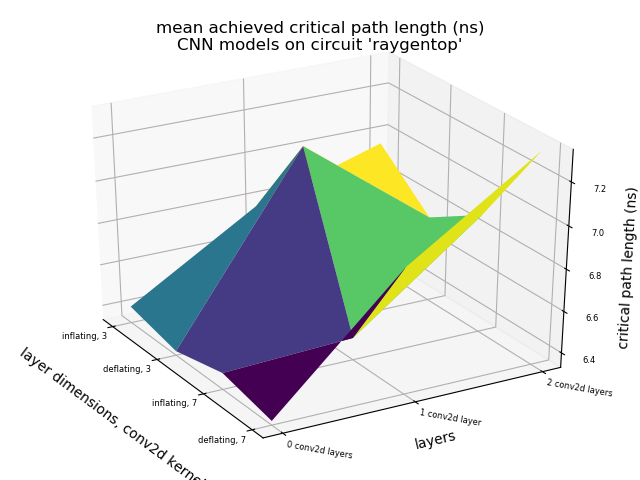
\includegraphics[width=\linewidth]{plots/cnn-hyperopt-critical-path.png}
		\caption{\glspl{CNN} - critical path length}
	\end{subfigure}
	\begin{subfigure}[b]{0.45\linewidth}
		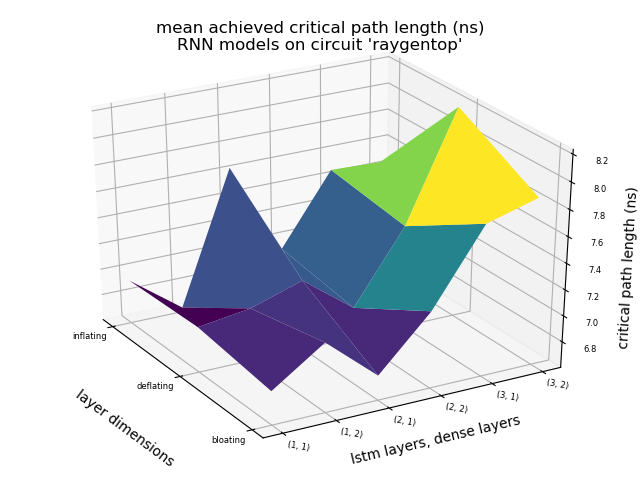
\includegraphics[width=\linewidth]{plots/rnn-hyperopt-critical-path.png}
		\caption{\glspl{RNN} - critical path length}
	\end{subfigure}
	\caption{Achieved performance over model configurations.}
	\label{fig:eval-hyperopt-surface}
\end{figure}

\begin{tabular}{lrrrrrrrrrr}
	\toprule
	conv\_layer\_count & \multicolumn{2}{l}{0} & \multicolumn{4}{l}{1} & \multicolumn{4}{l}{2} \\
	structure &  def &  inf & \multicolumn{2}{l}{def} & \multicolumn{2}{l}{inf} & \multicolumn{2}{l}{def} & \multicolumn{2}{l}{inf} \\
	kernel\_size &         -1 &         -1 &          3 &          7 &          3 &          7 &          3 &          7 &         3 &          7 \\
	\midrule
	channel\_width    &  11.0 &  10.3 &  19.4 &  17.9 &  19.2 &  19.5 &  19.6 &  18.3 &  19.6 &  20.1 \\
	critical\_path\_ns &  43.1 &  44.5 &  42.9 &  42.4 &  44.3 &  42.2 &  43.3 &  44.3 &  44.4 &  42.7 \\
	\bottomrule
	\label{TODO bad values}
	\label{table:cnn-hyperopt-results}
\end{tabular}

\begin{figure}
\begin{subfigure}[b]{0.45\linewidth}
	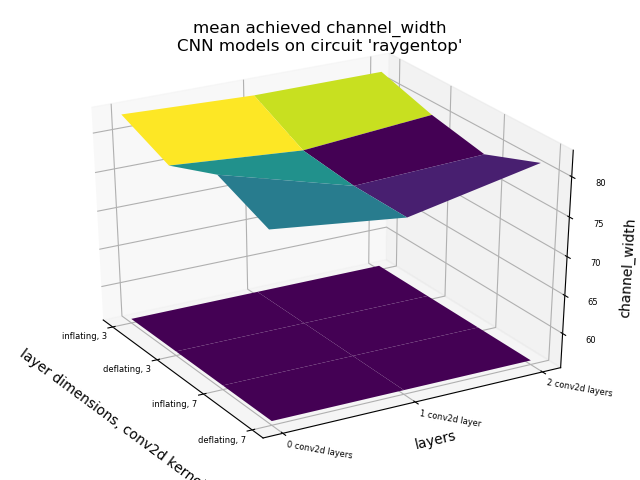
\includegraphics[width=\linewidth]{plots/cnn-hyperopt-chan-width-with-reference.png}
	\caption{\glspl{CNN} - channel width}
\end{subfigure}
\begin{subfigure}[b]{0.45\linewidth}
	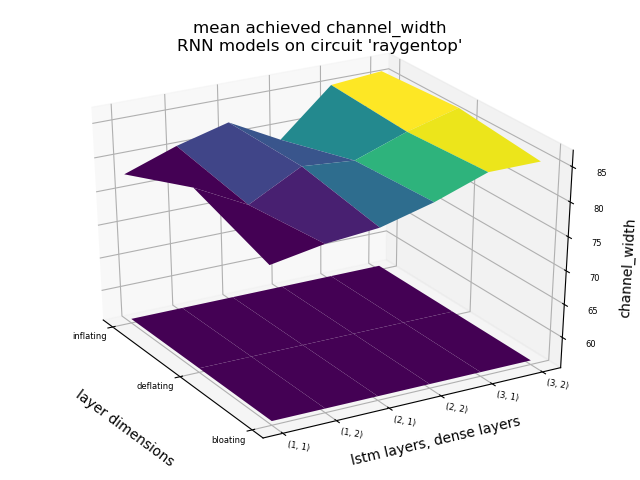
\includegraphics[width=\linewidth]{plots/rnn-hyperopt-chan-width-with-reference.png}
	\caption{\glspl{RNN} - channel width}
\end{subfigure}
\begin{subfigure}[b]{0.45\linewidth}
	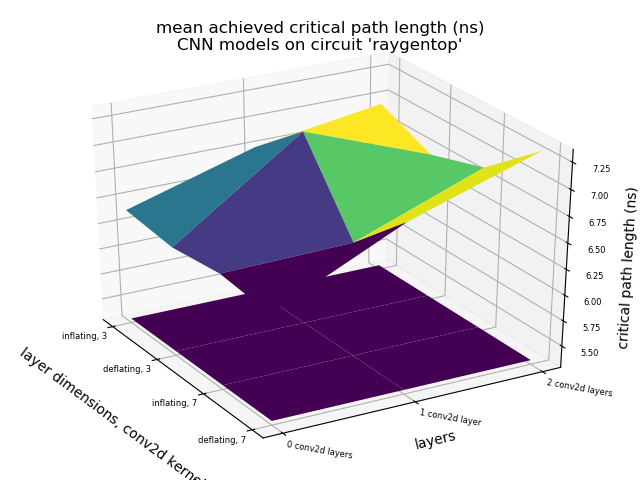
\includegraphics[width=\linewidth]{plots/cnn-hyperopt-critical-path-with-reference.png}
	\caption{\glspl{CNN} - critical path length}
\end{subfigure}
\begin{subfigure}[b]{0.45\linewidth}
	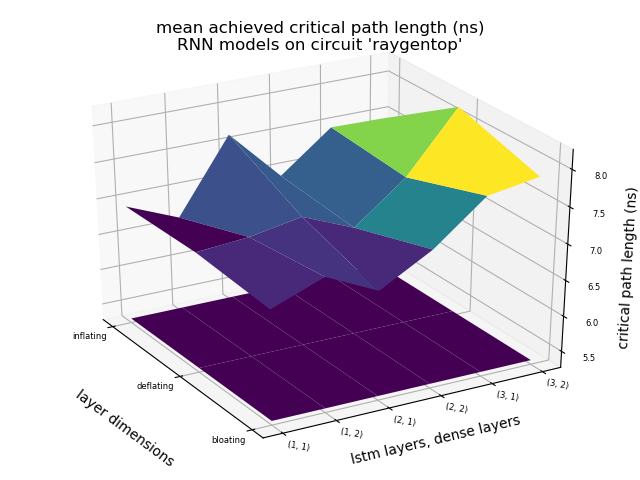
\includegraphics[width=\linewidth]{plots/rnn-hyperopt-critical-path-with-reference.png}
	\caption{\glspl{RNN} - critical path length}
\end{subfigure}
\caption{Achieved performance over model configurations with performance of reference system.}
\label{fig:eval-hyperopt-surface-reference}
\end{figure}

As these groups of candidates are generated from discrete parameters, e.g. dense layer count, this model selection approach constitutes a grid search over these hyperparameters.

By evaluating the \gls{NN} candidates on the evaluation set at the \textit{slow-mode} sampling point we determine their relative performance. A visualization of the results in \ref{fig:eval-hyperopt-surface} clearly shows a correlation between network complexity and routing quality: Smaller networks produce better results, with the exception of \glspl{CNN} without convolutional layers. These models, using less time for a prediction, allow for a higher number of moves per temperature step, although producing less accurate predictions than their more complex counterparts. The properties of convolutional layers, while computationally being rather expensive (at least compared to the "tiny" dense layers), seem to be beneficial to accurately predict the wiring cost. As the \gls{LSTM} layers of the \glspl{RNN} are required to encode the input data for the following dense layers, their suitedness to the problem can not be measured that easily.

The exact results are presented in \ref{table:rnn-hyperopt-results} and \ref{table:cnn-hyperopt-results}. We thus select \textit{1\_conv\_layers\_deflating\_kernel\_size\_7} and \textit{1\_lstm\_layers\_1\_dense\_layers\_inflating} as the best \gls{CNN} and \gls{RNN} models, respectively.

By comparing the performance to that of the unchanged \gls{VPR} Placer we can, however, also see, that none of the \glspl{NN} is able to beat \gls{HPWL} in \textit{slow-mode} (see \ref{fig:eval-hyperopt-surface-reference}).

\section{Results}

With a single network per type the modified \gls{VPR} Placer can now be evaluated against the unchanged version (reference system).

First, we present the performance of the reference system on our selected benchmarking test set. We then proceed by performing the same evaluation for our modified versions of the \gls{VPR} Placer, using \glspl{CNN} and\glspl{RNN}, respectively. A comprehensive comparison will answer the main question of this thesis, whether \gls{VPR} can be improved by replacing the crude \gls{HPWL} metric with more accurate, but also more expensive \glspl{NN}. Finally, we discuss our results and try to explain the observed behaviour.

\subsection{Reference System (Unchanged \gls{VPR})}

\subsection{\gls{CNN} Integration}

\subsection{\gls{RNN} Integration}

\subsection{Comparison}

\subsection{Justification}

covers discussion chapter?
